\section{Einleitung}
\label{sec:intro}

\subsection{Zweck}
Im vorliegenden Dokument sind die Anforderungen definiert, welche im Projekt \subjectinfo\ umgesetzt werden müssen. 
Es beschreibt den Auftrag zwischen Auftraggeber und Auftragnehmer. 
Der Ausdruck Pflichtenheft ist hier im Sinne der IEEE Recommended Practice for Software Requirements Specification. ANSI/IEEE Std 830-1998 verwendet.
Die dort definierte Requirements Specification beinhaltet sowohl die Benutzeranforderungen (Lastenheft gemäss DIN 69901-5) als auch Realisierungsvorgaben an die Entwicklungsgruppe (Pflichtenheft gemäss DIN 69901-5).

\subsection{Produktüberblick}
Im Rahmen dieses Projekt soll eine Software entwickelt werden, welche das optimale Spannungsteiler Widerstandsverhältnis für einen unbelasteten Spannungsteiler berechnet.
\begin{figure}[!h]
	\centering
	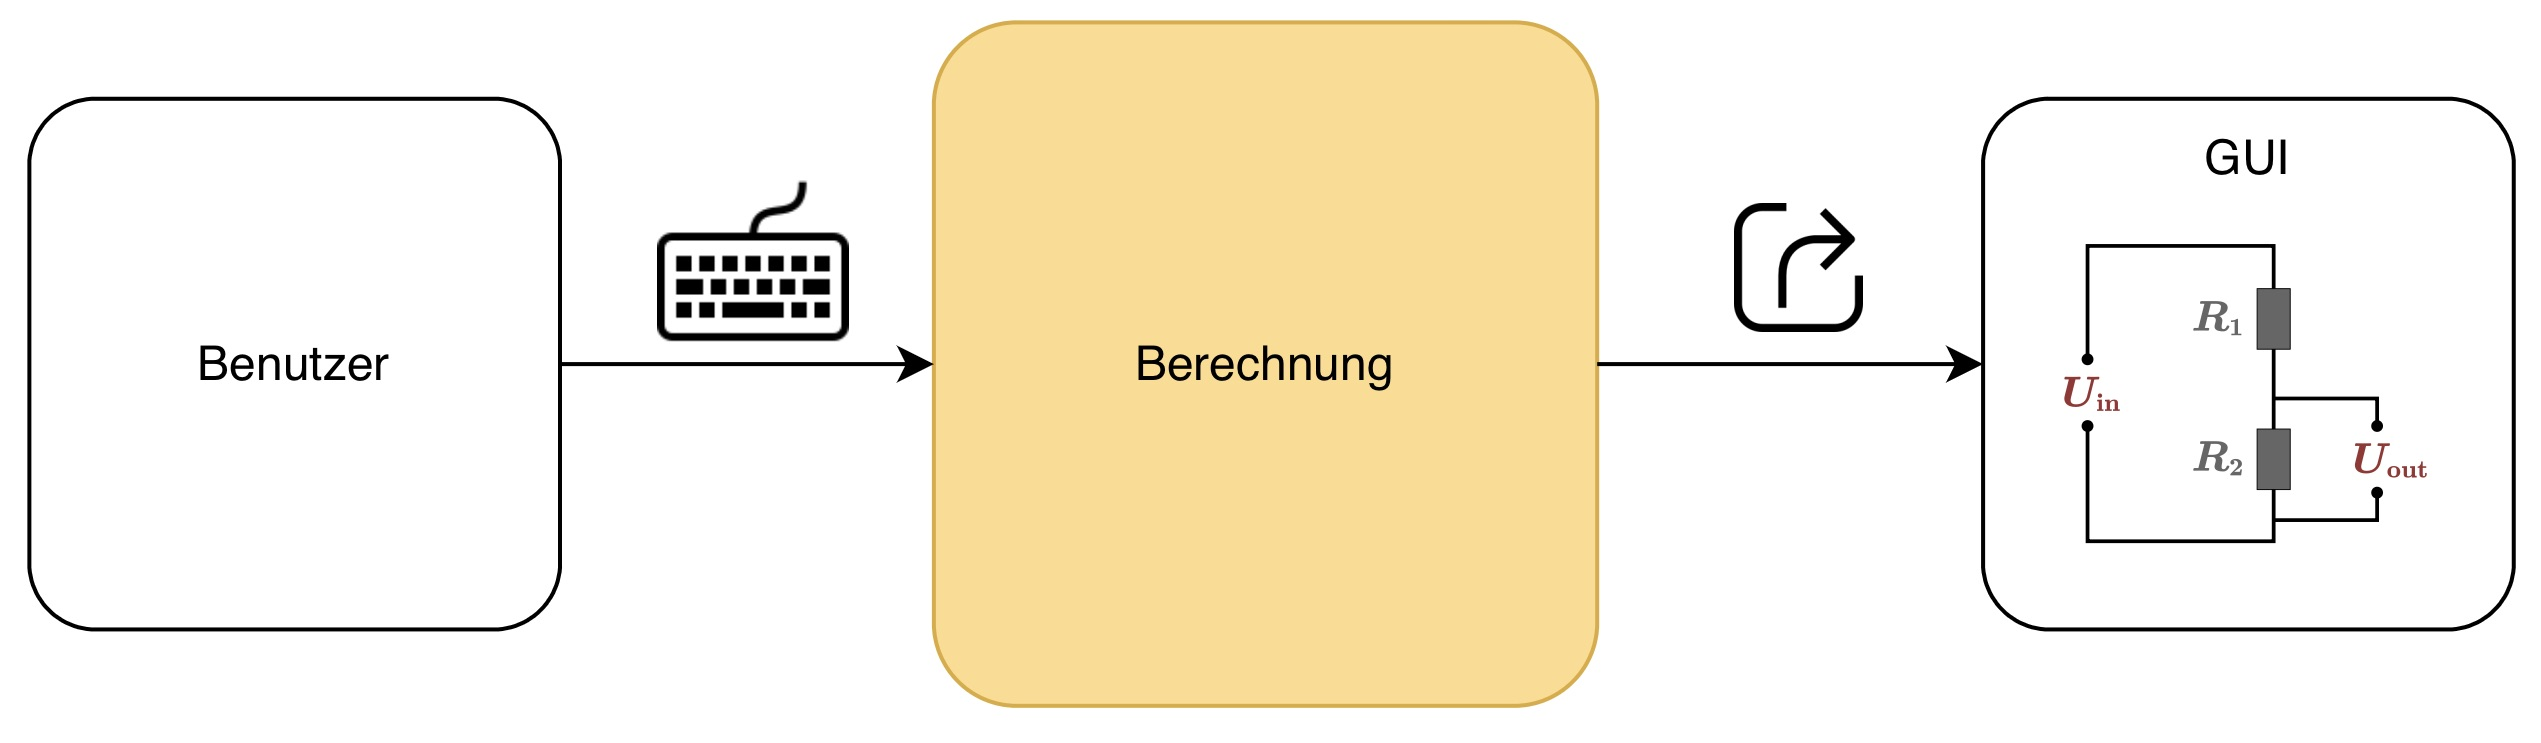
\includegraphics[width=12cm]{./images/Block.png}
	\caption{Blockschaltbild des Widerstands-Berechnungstools}
	\label{fig:blockdiagram}
\end{figure}

\subsection{Definitionen, Akronyme und Abkürzungen}
Keine
%\note{(Optional) Define all terms, acronyms, and abbreviations used in this document. This often goes into a separate document in a larger project.}

\subsection{Referenzen}
Siehe Anhang \ref{anx:ref} auf Seite \pageref{anx:ref} dieses Dokuments.